\section{Durchführung}
\label{sec:Durchführung}
\subsection{Auf- und Entladevorgang}
Um den Auf- und Entladevorgang zu untersuchen wird folgendes Schaltbild aufgebaut.
\begin{figure}[H]
    \centering
    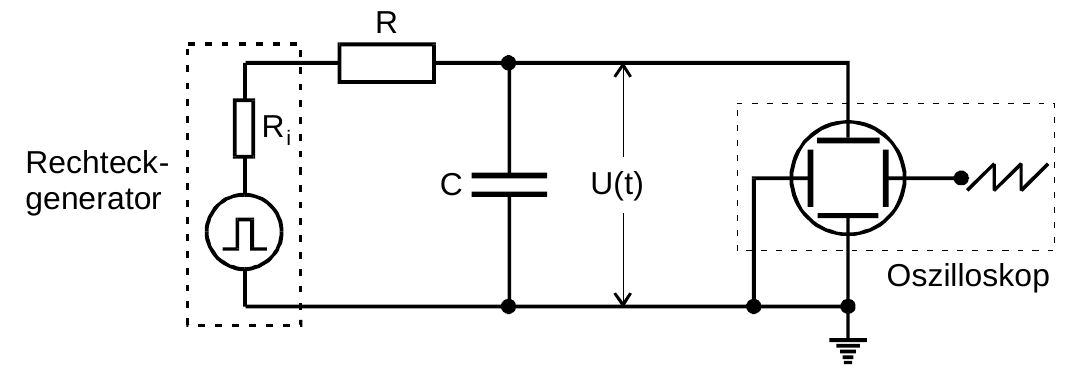
\includegraphics[width=\textwidth]{content/aufbau1.png}
    \caption{Aufbau der ersten Messung.\cite{v353}}
    \label{fig:mess1}
\end{figure}
\noindent
Dabei wird das RC-Glied an einen Rechteckgenerator angeschlossen und die resultierende Kondensatorspannung $U_C$ mit einem Oszilloskop beobachtet, sodass sich ein stationäres Bild einstellt. Die Spannung wird bei einer geeineten Frequenz zu mehreren Zeitpunkten innerhalb der Periode abgelesen.
Im Allgemeinen ist der Innenwiderstand des Generators zu beachten, welcher mit \mbox{$R_i=\SI{600}{\ohm}$\cite{v353}} angegeben ist. Wenn jedoch der Widerstand des RC-Glieds ausreichend hoch ist, kann ersterer vernachlässigt werden. Daher muss $R$ ausgemessen werden, um die Ergebnisse des Versuchs beurteilen zu können.
%
\subsection{Frequenzabhängigkeit der Amplitude}
Es wird die Frequenzabhängigkeit der Amplitude der Kondensatorspannung bei Sinusförmiger Anregung des RC-Glieds untersucht.
Dafür wird die Schaltung wie in Abbildung \ref{fig:mess2} gezeigt aufgebaut.
\begin{figure}[H]
    \centering
    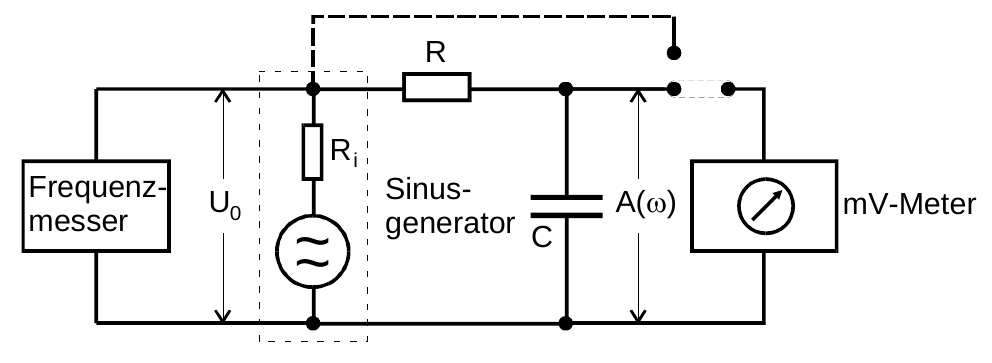
\includegraphics[width=\textwidth]{content/aufbau2.png}
    \caption{Aufbau der zweiten Messung.\cite{v353}}
    \label{fig:mess2}
\end{figure}
\noindent
Anstatt des Rechteckgenerators wird nun ein Sinusgenerator verwendet. Dieser wird im Verlauf der Messung auf verschiedene Frequenzen über mehrere Zehnerpotenzen hinweg eingestellt und die resultierende Amplitude der Kondensatorspannung gemessen.
Zusätzlich wird der Wiederstand des RC-Glieds mit einem digitalem Ohmmeter gemessen.
Auch hier ist der Innenwiderstand des Generators zu beachten.
%
\subsection{Frequenzabhängigkeit der Phasenverschiebung}
Im Gegensatz zur vorausgegangenen Messung wird nun auch die Generatorspannung gleichzeitig mit dem Oszilloskop beobachtet, sodass sich die Phasenverschiebung zwischen beiden messen lässt.
\begin{figure}[H]
    \centering
    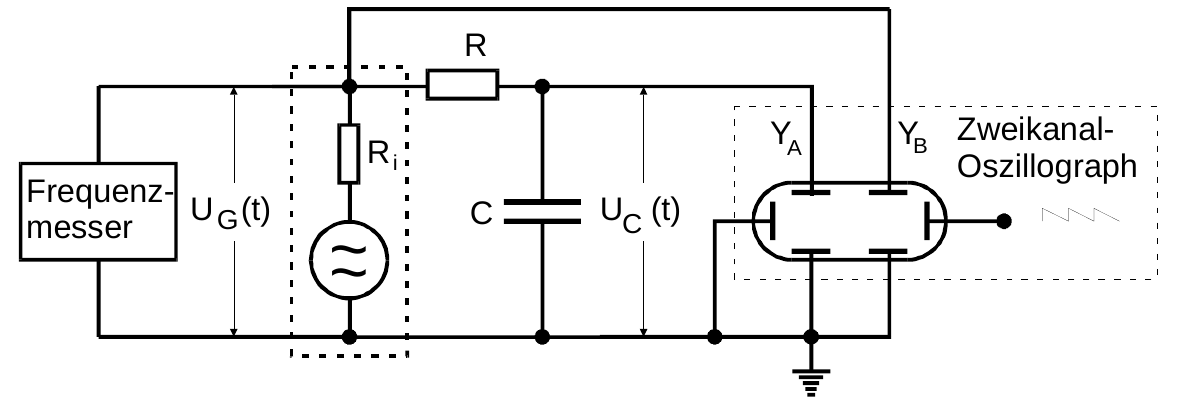
\includegraphics[width=\textwidth]{content/aufbau3.png}
    \caption{Aufbau der zweiten Messung.\cite{v353}}
    \label{fig:mess3}
\end{figure}
\noindent
Da sich der Phasenwinkel nicht direkt ablesen lässt wird einerseits der zeitliche Abstand zwischen zwei entsprechenden Nulldurchgängen beider Spannungssignale, hier $a$, und zusätzlich die gesamte Periode, hier $b$, gemessen, woraus sich der Phasenwinkel nach
\begin{equation}
    \phi = 2\pi \, \frac{a}{b}
    \label{eqn:abphase}
\end{equation}
ergibt.
Auch hier wird Frequenz des Generators im Verlauf der Messreihe über mehrere Zehnerpotenzen variiert.
